\documentclass[11pt, oneside]{article}   	% use "amsart" instead of "article" for AMSLaTeX format
\usepackage{geometry}                		% See geometry.pdf to learn the layout options. There are lots.
\geometry{letterpaper}                   		% ... or a4paper or a5paper or ... 
\usepackage{amsmath} 
\usepackage{amssymb}
%\geometry{landscape}                		% Activate for rotated page geometry
%\usepackage[parfill]{parskip}    		% Activate to begin paragraphs with an empty line rather than an indent
\usepackage{graphicx}				% Use pdf, png, jpg, or eps§ with pdflatex; use eps in DVI mode
\usepackage{subfigure}								% TeX will automatically convert eps --> pdf in pdflatex		
\usepackage{amssymb}
\usepackage{float}
%SetFonts

%SetFonts


\title{An HLL Riemann Solver for 1D MHD}
\author{Jiarong Zhu}
\date{}							% Activate to display a given date or no date

\begin{document}
\maketitle
In astrophysics, one often deals with ionized gas subject to magnetic field, so it's very useful to develop numerical methods to study the dynamical properties of magnetofluids. In this project, I realized a first order HLL approximate Riemann solver for one dimensional magneto hydrodynamics(MHD) equations and did several numerical tests. Some of the tests are standard MHD tests, so I compared them with results that already existed. Then I proceeded to develop high order scheme and compared the numerical results with what I've got in first order case. From the results we can see the first order HLL approximate Riemann solver works well for 1D MHD, but the resolution is not good enough, to improve resolution one has to resort to high order, or use other solvers such as HLLC solver, HLLD solver and the Roe solver. 

\section{Background}
 
\subsection{1D MHD equations}
We are considering non-relativistic case. To derive MHD equations, we need to combine hydrodynamics equations with Maxwell's equations. Rescale the magnetic field $B$ to be $B/2\pi$ for convenince, the three dimensional MHD equations are as follows:

\begin{equation}
\frac { \partial } { \partial t } \left[ \begin{array} { c } { \varrho } \\ { \varrho u } \\ { B } \\ { E } \end{array} \right] + \nabla \cdot \left[ \begin{array} { c } { \varrho u } \\ { \varrho u u + I \left( \left( p + \frac { 1 } { 2 } B ^ { 2 } \right) - B B \right) } \\ { u B - B u } \\ { \left( E + p + \frac { 1 } { 2 } B ^ { 2 } \right) u - B ( u \cdot B ) } \end{array} \right] = 0
\end{equation}
Where  total energy $E$ is given by

\begin{equation}
    E = \frac{p}{\gamma -1} +  \frac { 1 } { 2 } \rho v ^ 2 + \frac { 1 } { 2} B ^ { 2 }
\end{equation}
for gamma-law gas, which gives the expression of pressure:

\begin{equation}
    p = ( \gamma - 1 ) \left( E - \frac { 1 } { 2 } \rho v ^ { 2 } \right) - \frac { 1 } { 2 } B ^ { 2 }
\end{equation}
To derive one dimensional MHD equations, let all the variabes $u$ depend on x and t only, that's to make 
\begin{equation}
    \frac{\partial u}{\partial y} = \frac{\partial u}{\partial z}=0
\end{equation}
Then Eq.(1), Eq.(4) and $\nabla \cdot B = 0$ give us $B_x = constant$. Now the 1D MHD equations are :
\begin{equation}
  \frac { \partial } { \partial t } \left[ \begin{array} { c } { \rho } \\ { \rho v _ { x } } \\ { \rho v _ { y } } \\ { \rho v _ { z } } \\ { B _ { y } } \\ { B _ { z } } \\ { E } \end{array} \right] + \frac { \partial } { \partial x } \left[ \begin{array} { c } { \rho v _ { x } } \\ { \rho v _ { x } ^ { 2 } + p + \frac { 1 } { 2 } B ^ { 2 } - B _ { x } ^ { 2 } } \\ { \rho v _ { x } v _ { y } - B _ { x } B _ { y } } \\ { \rho v _ { x } v _ { z } - B _ { x } B _ { z } } \\ { B _ { z } v _ { x } - B _ { x } v _ { z } } \\ { B _ { z } v _ { x } - B _ { x } v _ { z } } \\ { v _ { x } \left( E + p + \frac { 1 } { 2 } B ^ { 2 } \right) - B _ { x } \left( v _ { x } B _ { x } + v _ { y } B _ { y } + v _ { z } B _ { z } \right) } \end{array} \right] = 0  
\end{equation}
This is the main equation to be used in our numerical scheme. Note that this equation has the form of conservation law:
\begin{equation}
    \frac{\partial \textbf{U}}{\partial t} + \frac{\partial \textbf{F}}{\partial x} = 0
\end{equation}


\subsection{Wave structure of 1D MHD equations}
Eq.(6) can also be written in the form:
\begin{equation}
    \partial _ { t } \mathbf { U } + \mathbf { A } \cdot \partial _ { x } \mathbf { U } = 0
\end{equation}
where $\mathbf{A}$ denotes Jacobian matrix of the PDE system. As $\mathbf{A}$ is diagonalizable with real eigenvalues, so the MHD equation is hyperbolic. Diagonalize $\mathbf{A}$, the Eq.(7) becomes a set of decoupled linear advection equations, with the eigenvalues being corresponding wave speeds. Solving for eigenvalues of $\mathbf{A}$ gives seven wave speed as below:

\begin{equation}
\begin{array} { l } { \lambda _ { 1,7 } = u \mp c _ { f } } \\ { \lambda _ { 2,6 } = u \mp c _ { a } } \\ { \lambda _ { 3,5 } = u \mp c _ { s } } \\ { \lambda _ { 4 } = u } \end{array}
\end{equation}

Where 
\begin{equation}
\begin{aligned} c _ { f , s } ^ { 2 } = \frac { 1 } { 2 } \left[ \left( a ^ { 2 } + v _ { A } ^ { 2 } \right) \right. & \pm \sqrt { \left( a ^ { 2 } + v _ { A } ^ { 2 } \right) ^ { 2 } - 4 a ^ { 2 } c _ { a } ^ { 2 } } ] \\ c _ { a } & = \frac { B _ { x } } { \sqrt { 4 \pi \rho } } \\ v _ { A } & = \frac { B } { \sqrt { \frac { \gamma P } { \rho } } } \\ a & = \sqrt { \frac { \gamma P } { \rho } } \end{aligned}
\end{equation}

We observe that the eigenvalues follow sequence as:
$\lambda_1 \leq \lambda_2 \leq ... \leq \lambda_6 \leq \lambda_7$.
These speeds are defined as below: $\lambda_{1,7}$ are fast magnetosonic waves, $\lambda_{3,5}$ are slow magnetosonic waves. These magnetosonic waves in Riemann problem typically will have shock or rarefaction wave solutions.$\lambda_{3,5}$ are called  Alfven  waves, which are purely transverse waves, with $\rho,v_x,p$ being constant while transverse magnetic field and transverse velocities vary. These waves will be shown in our numerical tests. Figure.1 shows the space-time diagram of MHD waves.

\begin{figure}[H]
\centering
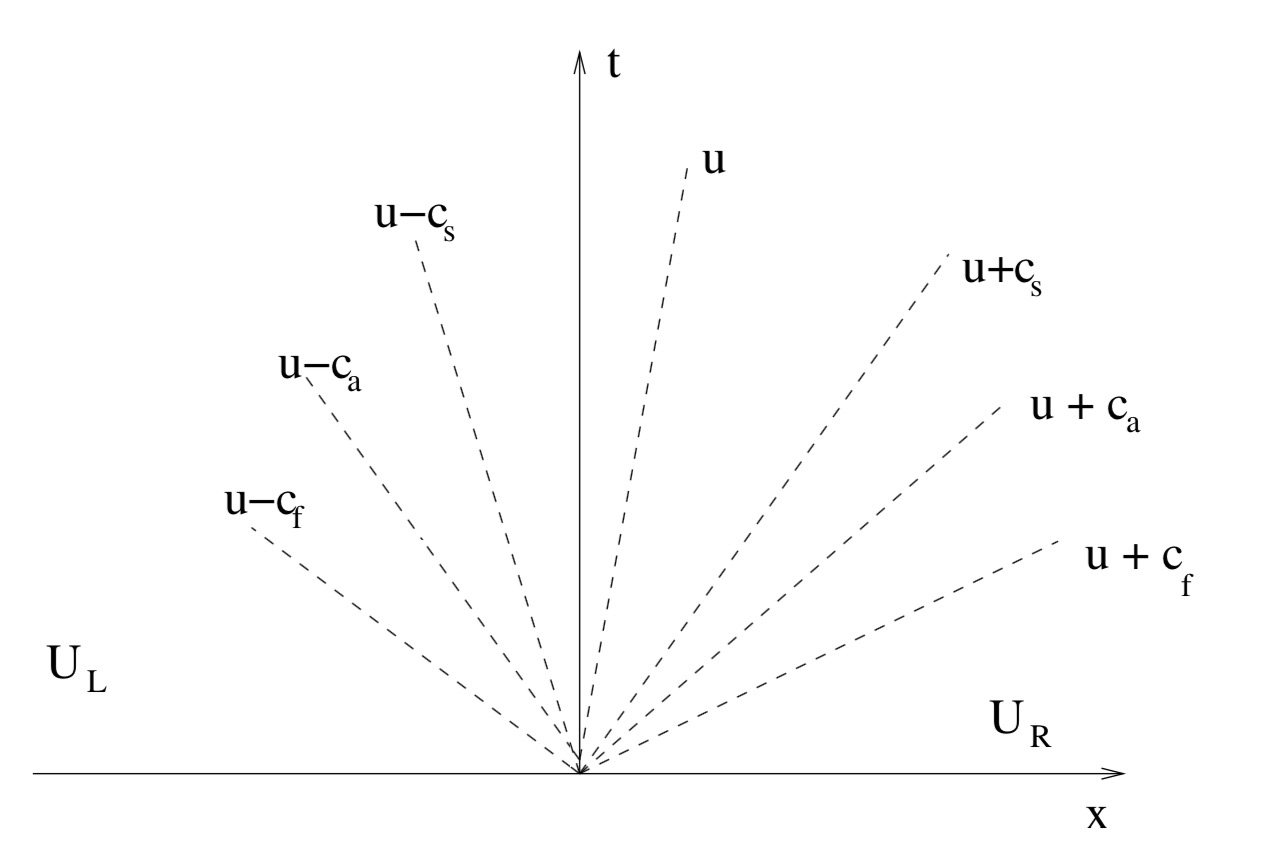
\includegraphics[scale = 0.2]{wave_structure.png}
\caption{Waves in 1D MHD Riemann problem}
\end{figure}


\section{Numerical methods}
\subsection{First order Scheme}
I adopted the numerical scheme used in hydrodynamics. By discretizing Eq.6, we get expression as:
\begin{equation}
    \mathbf { U } ^ { n + 1 } = \mathbf { U } ^ { n } - \frac { \Delta t } { \Delta x } \left( \mathbf { F } _ { i + 1 / 2 } ^ { n } - \mathbf { F } _ { i - 1 / 2 } ^ { n } \right)
\end{equation}
The superscript denotes time, while the subscript denotes position. So we can use this formula to update all variable values after time $\Delta t$. The flux at interface is unknown, we estimate it by using HLL flux:
\begin{equation}
    \mathbf { F } ^ { \mathrm { HLL } } = \frac { \alpha ^ { + } \mathbf { F } ^ { \mathrm { L } } + \alpha ^ { - } \mathbf { F } ^ { \mathrm { R } } - \alpha ^ { + } \alpha ^ { - } \left( \mathbf { U } ^ { \mathrm { R } } - \mathbf { U } ^ { \mathrm { L } } \right) } { \alpha ^ { + } + \alpha ^ { - } }
\end{equation}
where $\alpha ^ { + },\alpha ^ { - }$are given by:
\begin{equation}
    \alpha ^ { \pm } = \operatorname { MAX } \left\{ 0 , \pm \lambda ^ { \pm } \left( \mathbf { U } ^ { \mathrm { L } } \right) , \pm \lambda ^ { \pm } \left( \mathbf { U } ^ { \mathrm { R } } \right) \right\}
\end{equation}
\begin{equation}
    \lambda ^ { \pm } = v_x \pm c _ { f }
\end{equation}
As fast magnetosonic waves are the fastest among all wave speeds.
$\Delta t$ must satisfy CFL condition, so we set it to be:

\begin{equation}
    \Delta t = CFL * \frac{\Delta x}{ \mathrm { MAX } ( \alpha ^ { \pm })} 
\end{equation}
The CFL number is between 0 and 1.

\subsection{High order scheme}
In the high order scheme, the time integration is realized by using RK3, thus it is third order accurate. The formula is something we're familiar with:
\begin{equation}
    \begin{aligned} \mathbf { U } ^ { ( 1 ) } & = \mathbf { U } ^ { n } + \Delta t L \left( \mathbf { U } ^ { n } \right) \\ \mathbf { U } ^ { ( 2 ) } & = \frac { 3 } { 4 } \mathbf { U } ^ { n } + \frac { 1 } { 4 } \mathbf { U } ^ { ( 1 ) } + \frac { 1 } { 4 } \Delta t L \left( \mathbf { U } ^ { ( 1 ) } \right) \\ \mathbf { U } ^ { n + 1 } & = \frac { 1 } { 3 } \mathbf { U } ^ { n } + \frac { 2 } { 3 } \mathbf { U } ^ { ( 2 ) } + \frac { 2 } { 3 } \Delta t L \left( \mathbf { U } ^ { ( 2 ) } \right) \end{aligned}
\end{equation}
To make it high order in space, I still used the piecewise linear reconstruction. The slope limiter $\theta $ has a crucial influence in the outcome. I'll show this in the numerical test results.

\subsection{HLLC Riemann solver}
There are different types of Riemann solvers. In HLL Riemann solver, only the fastest waves are maintained, with all intermediate states averaged to be one state. HLLC, HLLD and Roe solver keeps other waves, making the resolution higher and less diffusive. Fig.2 gives a conceptual description of these methods:

\begin{figure}[H]
\centering
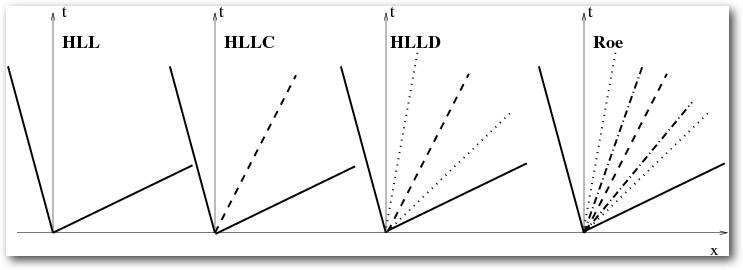
\includegraphics[scale = 0.4]{riemann_solvers.png}
\caption{Different Riemann solvers}
\end{figure}

In my project, I tried to realize HLLC Riemann solver, which has two intermediate states in between, with the assumption that the intermediate left and right states share the same pressure and velocity. Unfortunately my code didn't work well, so I will not present any result of this part.

\section{Numerical Tests}
\subsection{First order tests}
\subsubsection{Brio-Wu test}
The left state is set to be:  $(\rho, vx, vy, vz, By, Bz, p) = (1,0,0,1,0,1)$ , and the right state: (0.125,0,0,-1,0,0.1). $\gamma = 2.0$, $B_x = 0.75$, CFL = 0.475, tfinal = 0.2, Nx = 2000.  Results are shown in Fig.3. Compared with results computed with Athena using the second order Roe solver, which are shown in Fig.4, we can see that our scheme works well.

\begin{figure}[H]

\subfigure[$\rho-x$]{
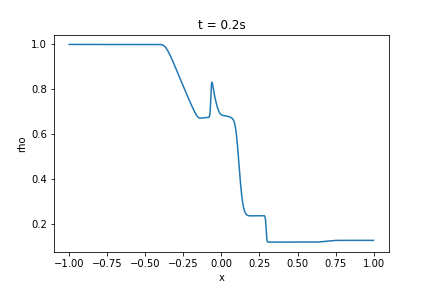
\includegraphics[scale=0.3]{rho.png}}
\subfigure[$v_x - x$]{
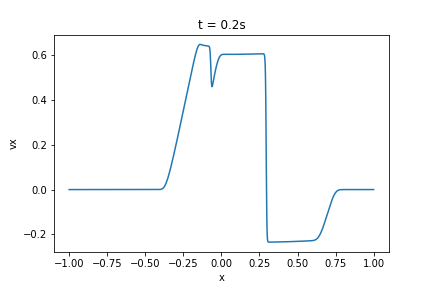
\includegraphics[scale=0.3]{vx.png}}
\subfigure[$v_y - x$]{
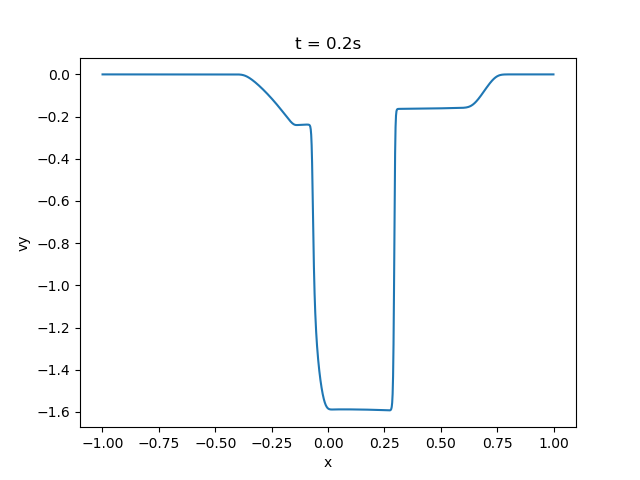
\includegraphics[scale=0.25]{vy.png}}
\subfigure[$B_y - x$]{
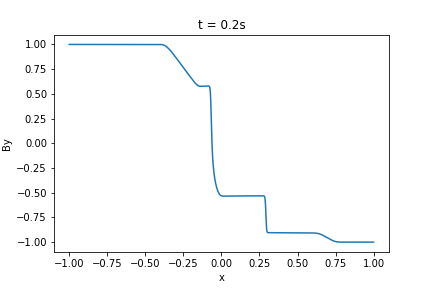
\includegraphics[scale=0.32]{By.png}}
\subfigure[p - x]{
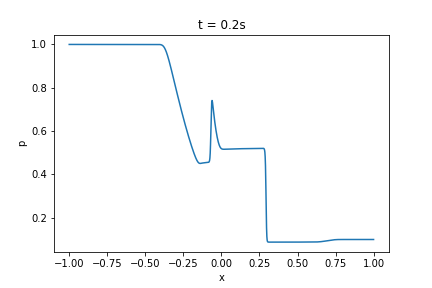
\includegraphics[scale=0.32]{p.png}}

\caption{Brio-Wu test results of the first order scheme, $Bz-z$ and $v_z$ do not vary, so I did not present them. From these figures, we can observe a fast rarefaction region, a compound wave composed of slow shock and rarefaction, a contact discontinuity, slow shock and a fast rarefaction region from left to right.}

\end{figure}

\begin{figure}[H]
\centering
\includegraphics[scale = 0.3]{brio_athena.png}
\caption{Brio-Wu shock tube test computed with Athena}
\end{figure}


\subsubsection{Hydrodynamic limit}
When we set the magnetic field to be 0, the MHD equations should reduce to Euler equations, then the magneto fluid would be the same as Euler fluid. I used same $\rho,p$ initial conditions as in Brio-Wu test, with magnetic field being zero. The outputs of MHD code and hydro code are presented in Fig.5, which are exactly the same, as we expected.

\begin{figure}[H]
\centering
\subfigure[Result by MHD code]{
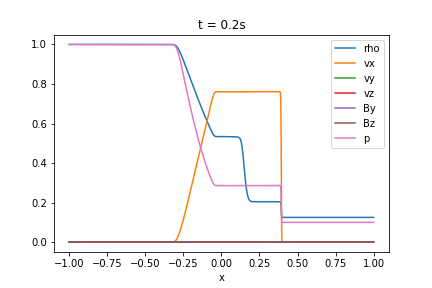
\includegraphics[scale=0.45]{3.png}}
\subfigure[Result by hydro code ]{
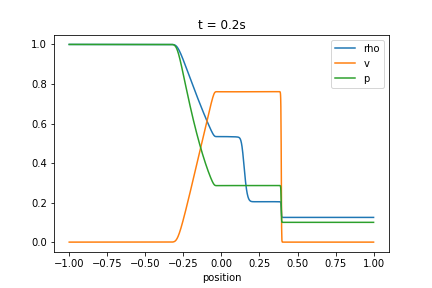
\includegraphics[scale=0.45]{all_euler.png}}
\caption{Magneto fluid reduces to Euler fluid}
\end{figure}

\subsubsection{Magnetic field is transverse}
In this case, $B_x = 0, B_y $ or $ B_z \neq 0$, then $c_f \neq 0, c_s = c_A = 0$, which means that the Alfven waves, slow waves and contact discontinuity collapse into a contact discontinuity as in Euler equations. The fast waves are acoustic, with the wave structure and speed being influenced by the transverse magnetic field. To verify this effect, I made $B_y = 1.0, B_x = B_z = 0$, $p_{left} = 1.0, p_{right} = 0.5, \rho_{left} = 0.2, \rho_{right} = 0.1, \gamma = 2.0, CFL = 0.475, tfinal = 0.2$. I got Fig.6:

\begin{figure}[H]
\centering
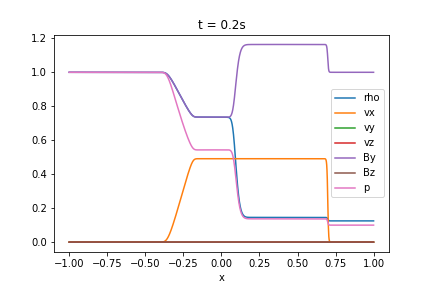
\includegraphics[scale = 0.6]{2.png}
\caption{1D MHD Riemann problem with transverse magnetic field, we can observe fast magnetosonic waves on both sides, and a contact discontinuity in the middle. }
\end{figure}

\subsubsection{Magnetic field is in the x-direction}
$B_x \neq 0, B_y = B_z = 0$. In this case, neither fast nor slow magnetosonic waves degenerates to an Alfven wave. Here I made a test when $B_x > a$, where $a$ is the sound speed, then we have $c_f = a, c_s = c_A = B_x$, i.e. the slow magnetosonic wave degenerates to Alfven wave, while the fast magnetosonic wave is acoustic. The left state is   $(\rho, vx, vy, vz, By, Bz, p) = (0.5,0,0.1,0,0,1.0)$ , and the right state: (0.1,0,0,0,0,0.2),$\gamma = 2.0, CFL = 0.475, tfinal = 0.1$, the results are as follows:

\begin{figure}[H]
\centering
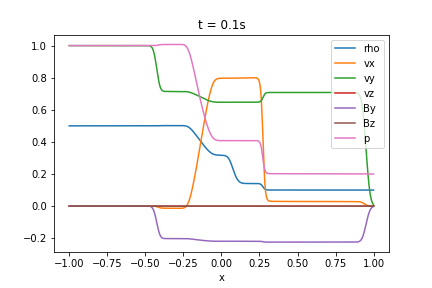
\includegraphics[scale = 0.6]{5.png}
\caption{1D MHD Riemann problem with magnetic field in x - direction, from left to right: Alfven(fast) wave, slow wave, contact discontinuity, slow wave, Alfven(fast) wave}
\end{figure}

\subsection{High order scheme}
\subsubsection{Brio-Wu test}
When choosing different slope limiter $\theta$, the high order scheme shows different level of instability. I show this by applying different value of $\theta$ in doing Brio-Wu test, giving results in Fig.8:


\begin{figure}[H]
\centering
\subfigure[$\theta = 1.5$]{
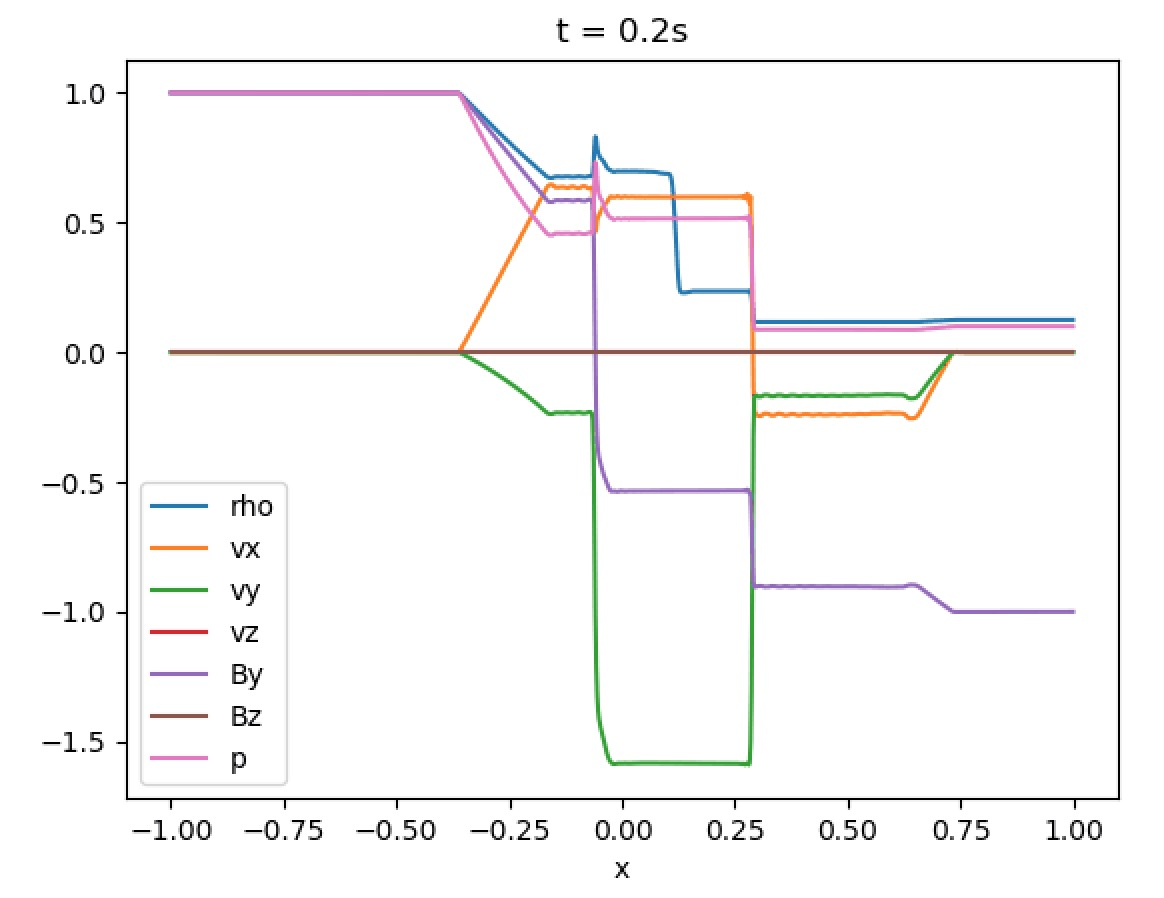
\includegraphics[scale=0.15]{Brio_highorder.png}}
\subfigure[$\theta = 1.0$ ]{
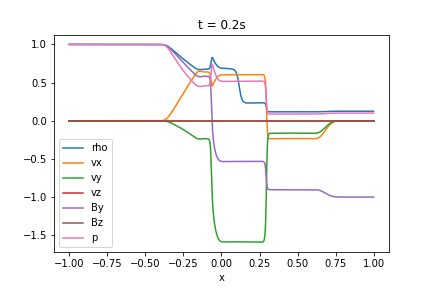
\includegraphics[scale=0.5]{Brio_high.png}}
\caption{High order scheme test with different $\theta$, we observe that with $\theta = 1$, the instability in (a) disappears }
\end{figure}

\subsubsection{Ryu and Jones test 2A}
With this test, I want to show that high order scheme has a higher resolution rather than first order scheme. I use 2000 cells in first order scheme to get (a), and 500 cells in high order scheme to get (b), with $\theta = 1.0$. Other parameters are:  Left state:$ (\rho, v_x, v_y, v_z, B_y, B_z, E) = (1.08, 1.2, 0.01, 0.5, 3.6/\sqrt{4\pi},2\sqrt{4\pi},0.95) $,Right state: $(\rho, v_x, v_y, v_z, B_y, B_z, E) = (1,0,0,0,4/\sqrt{4\pi},2/\sqrt{4\pi},1),
\\ B_x = 2/\sqrt{4\pi}, \gamma = 5/3, tfinal = 0.2s$. Also, this test is good because we can observe all 7 waves in this single test.

\begin{figure}[H]
\centering
\subfigure[First order result]{
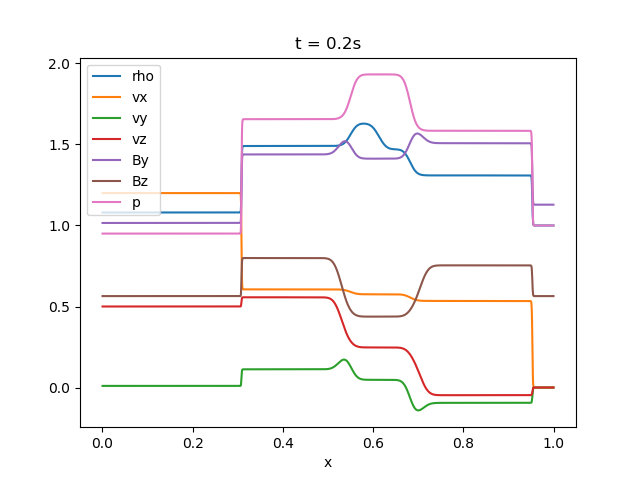
\includegraphics[scale=0.43]{RJ.png}}
\subfigure[High order result]{
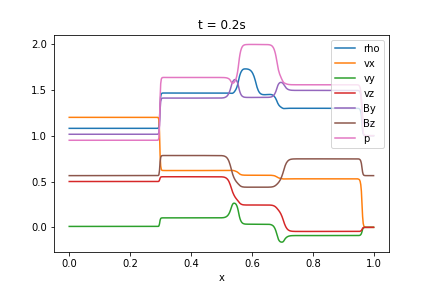
\includegraphics[scale=0.49]{RJ_highorder.png}}
\caption{First order scheme compared with high order scheme }
\end{figure}


\section{Conclusion and future work}
In this project, I realized both first order and high order ( 2nd order in space, 3rd order in time) HLL Riemann solver for one dimensional MHD equations as well as doing some numerical tests to see the behavior of physical properties of the system. There are many future work that can be done. For example, realizing other Riemann solvers such as HLLC, HLLD Riemann solver, which takes more intermediate states into consideration and should result in better resolution. One the other hand, it is necessary to expand the numerical solver into higher dimension like 2D or 3D, since the magneto fluid in real situation are always in three dimension.

\begin{thebibliography}{}
\bibitem{ref1}R. J. LeVequeD. MihalasE. A. DorfiE. Müller,1997,Computational Methods for Astrophysical Fluid Flow
\bibitem{ref2} Eleuterio F. Toro, Riemann Solvers and Numerical Methods for Fluid Dynamics.Third Edition
\bibitem{ref3}Shengtai Li, An HLLC Riemann solver for magneto-hydrodynamics, Journal of Computational Physics, v.203 n.1, p.344-357, 10 February 2005
\bibitem{ref4} TTakahiro Miyoshi , Kanya Kusano, A multi-state HLL approximate Riemann solver for ideal magnetohydrodynamics, Journal of Computational Physics, v.208 n.1, p.315-344, 1 September 2005 
\end{thebibliography}
\end{document}  